\model{Array Lists}

Arrays store elements in one \emph{contiguous} block of memory.
Since elements are stored together, you can immediately access any element by its index.

\vspace{1ex}
\begin{minipage}{0.50\linewidth}
\begin{javalst}
    int[] numbers = {22, 6, 14};
    System.out.println(numbers[1]);
\end{javalst}
\end{minipage}
\hfill
\begin{minipage}{0.48\linewidth}
\centering
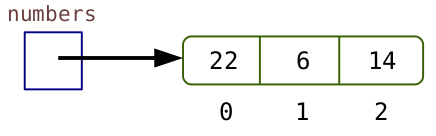
\includegraphics[scale=0.35]{figs/array1.png}
\end{minipage}
\vspace{1ex}

The \java{ArrayList} collection implements \java{List} and uses an array (internally) to store its elements.

\vspace{1ex}
\begin{minipage}{0.35\linewidth}
\begin{javalst}
    ArrayList<Integer> numbers = new ArrayList<>();
    numbers.add(22);
    numbers.add(6);
    numbers.add(14);
\end{javalst}
\end{minipage}
\hfill
\begin{minipage}{0.63\linewidth}
\vspace*{2em}
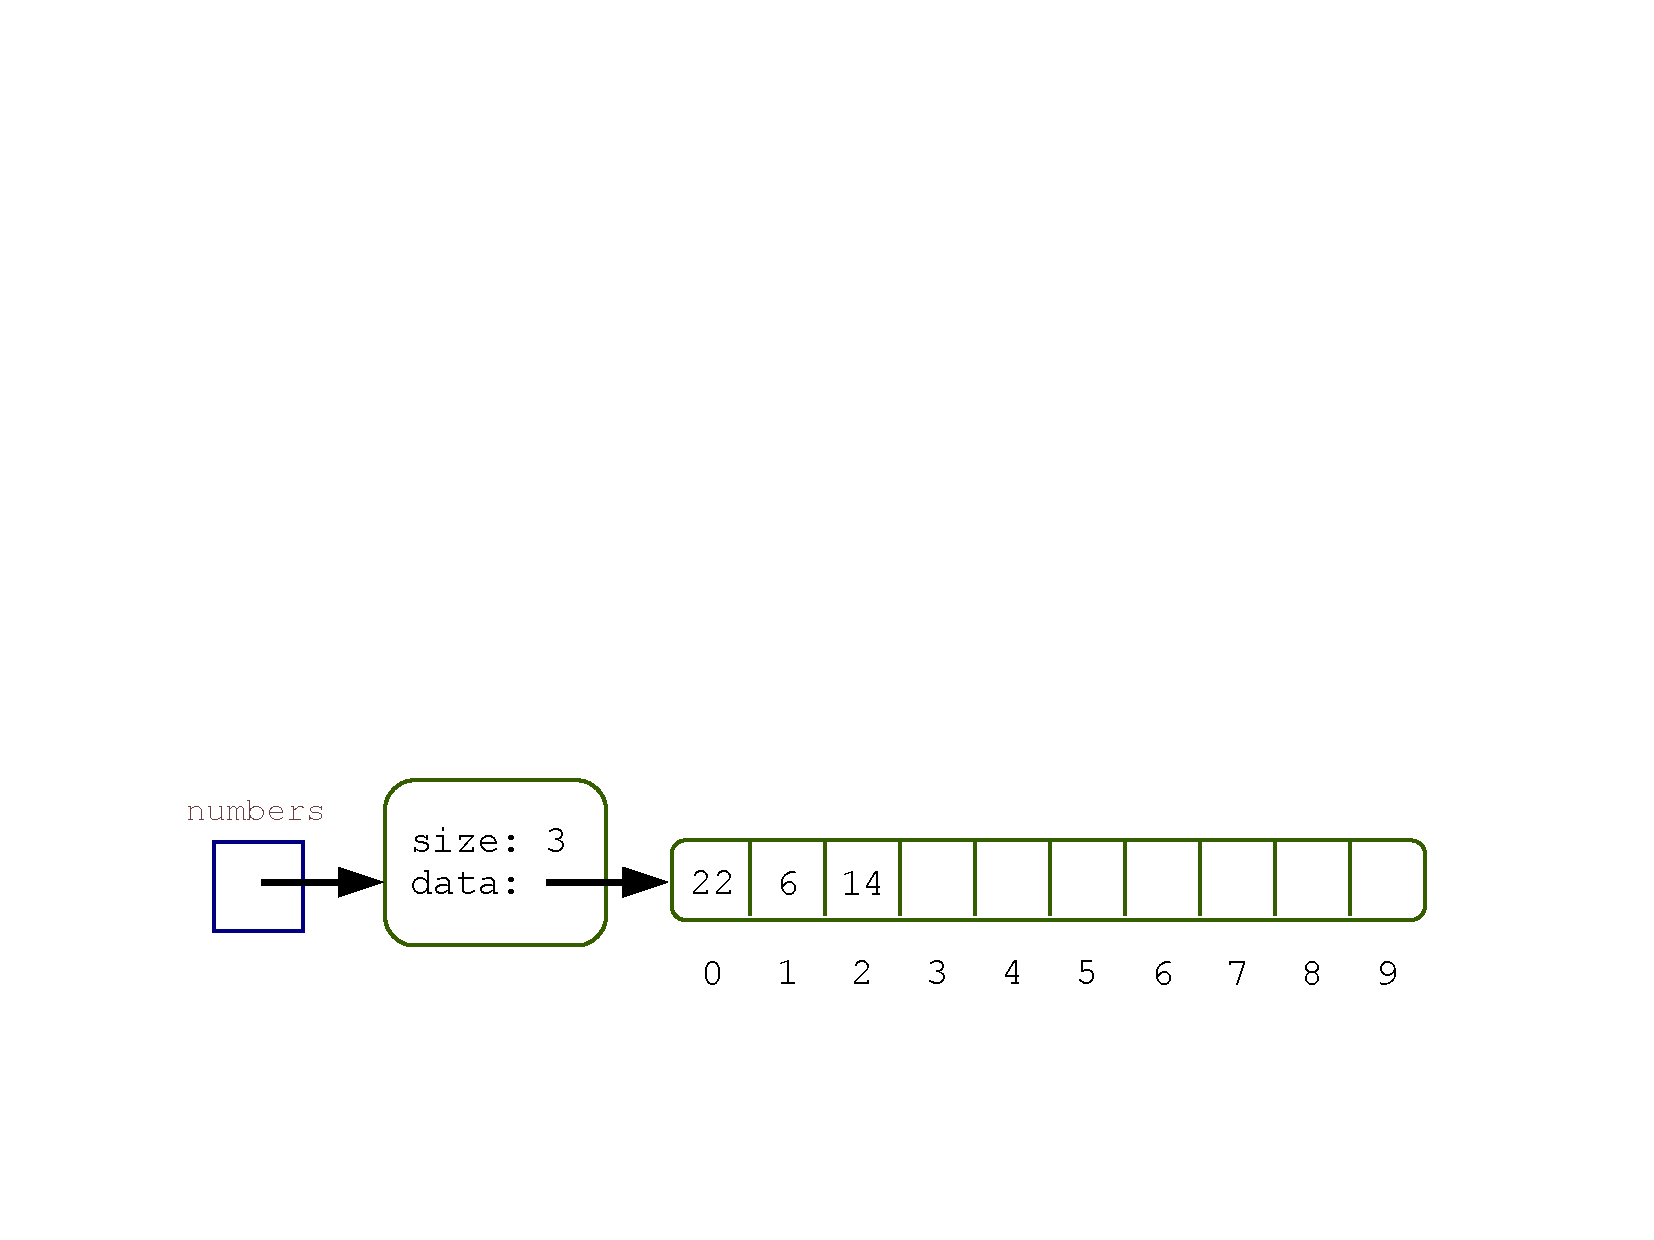
\includegraphics[scale=0.45]{figs/array2.pdf}
%Note these figures have 10 elements because that is the default for an ArrayList
\end{minipage}
\vspace{1ex}

When new values are inserted, existing array elements are moved to the right.

\vspace{1ex}
\begin{minipage}{0.35\linewidth}
\begin{javalst}
    numbers.add(0, 49);
    numbers.add(0, 74);
\end{javalst}
\end{minipage}
\hfill
\begin{minipage}{0.63\linewidth}
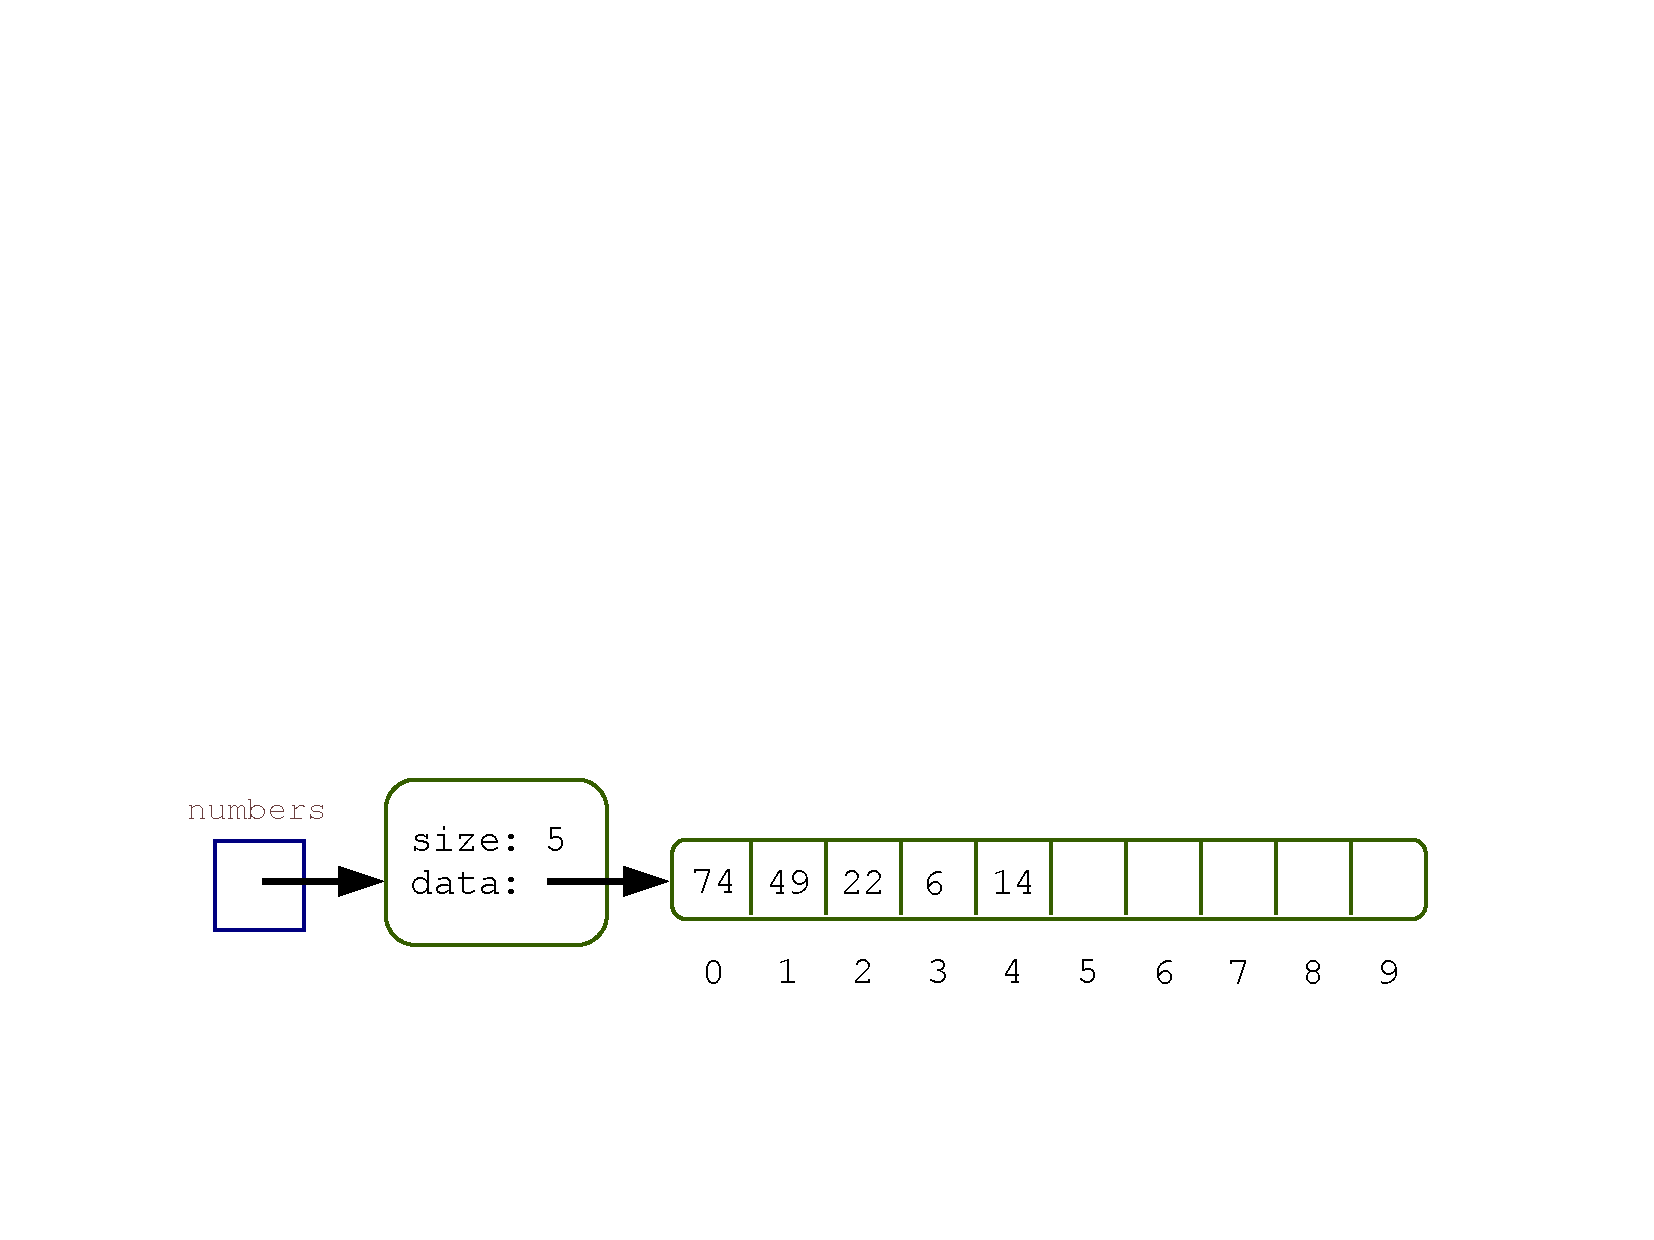
\includegraphics[scale=0.45]{figs/array3.pdf}
\end{minipage}
\vspace{1ex}

If the array fills up, \java{ArrayList} automatically creates a new array about 50\% larger.
All current values must be copied into the new array, and the old array is then garbage collected.


\quest{15 min}


\Q Why does Java use the name \java{ArrayList}?
(What do the words \java{Array} and \java{List} indicate?)

\begin{answer}
The \java{ArrayList} collection implements the \java{List} interface using an array.
In general, the first word tells how it's implemented, and the second word is the interface.
\end{answer}


%CSM let's not go here; the model hides details of autoboxing
%\Q How much memory is needed for each element in the array?
%
%\begin{answer}
%Each element takes the number of bytes of the size of the element.
%Here it is an Integer object, so 8 bytes for the reference, 16 bytes of object %overhead, and 4 bytes for the actual int.
%\end{answer}


\Q \label{arrayopers}
How many array operations (i.e., integer assignments) were required to add 49 and 79 to the front of the second diagram in \ref{\currfilename}?

\begin{answer}
There are 9 total array operations:
adding 49 takes 4 operations (3 shifts + 1 add), and adding 74 takes 5 operations (4 shifts + 1 add).
\end{answer}


\Q Imagine the internal array for \java{numbers} is full (i.e., with size=10 above).
If you request one more element to be added (at the end), how big will the new array be?

\begin{answer}
50\% of 10 is 5, so the new array will be 15 elements.
\end{answer}


\Q Continuing the previous question, what operations are required to add one more element when the array is full? Briefly describe each operation, beginning with creating the new array.

\begin{answer}[5em]
First, a new array of length 15 must be created.
Then, the 10 elements must be copied from the old array to the new array.
Next, the new element is added to the end and the \java{size} attribute is incremented.
Finally, the old array is garbage collected.
\end{answer}


\Q \label{ArraysAreBad}
Discuss why \java{ArrayList} is a poor choice of \java{List} in the program below:

\begin{quote}
\jafile{ArraysAreBad.java}
\end{quote}
\vspace{-1em}

\begin{answer}
Each insertion at the beginning of the array takes $n$ operations (where $n$ is the current size of the collection) in order to shift existing elements down.
\end{answer}


\Q \label{key2}
Arrays are simple and effective. Why would we want anything but ArrayList?

\begin{answer}
Arrays are inefficient when adding and removing items from the beginning (or the middle).
\end{answer}
